\documentclass[11pt,fleqn]{article}

\setlength {\topmargin} {-.15in}
\setlength {\textheight} {8.6in}

\usepackage{amsmath}
\usepackage{amssymb}
\usepackage{color}
\usepackage{tikz}
\usetikzlibrary{automata,positioning,arrows}
\usepackage{diagbox}
\usepackage{stackrel}
\begin{document}


\textbf{Exercise 1.3.46:} Forbidden triple for stack generability. Prove that a permutation can be generated
by a stack (as in the previous question) if and only if it has no forbidden triple (a, b,
c) such that a < b < c with c first, a second, and b third (possibly with other intervening
integers between c and a and between a and b).\\

\textbf{solution:} Suppose that there is a forbidden triple (a, b, c). Item c is popped before
a and b, but a and b are pushed before c. Thus, when c is pushed, both a and b are on
the stack. Therefore, a cannot be popped before b.\\

\begin{itemize}
	\item Numbers are pushed onto stack in accending order.
	\item stacks are LIFO(Last-in-first-out), so items must be popped in descending order.
	\item If $a<b$, "a" cannot be above "b" on the stack.
	\item Therefore, a permutation would not exist when a forbidden triple exists as it contradicts the structure of a stack.
\end{itemize}

The point c is needed so that after a pop, you can verify if order of a and b are correct(ascending) for a stack. Otherwise, it's hard to tell.


\begin{center}
	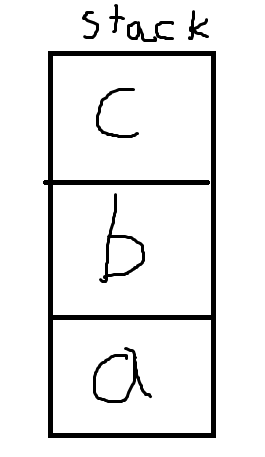
\includegraphics[scale = 1]{1.3.46.png}
	\end{center}

\end{document}
